\documentclass[11pt]{article}
\usepackage{amsmath,amssymb,amsmath,amsthm,amsfonts}
\usepackage{latexsym,graphicx}
\usepackage{fullpage,color}
\usepackage{url,hyperref}
\usepackage{natbib}
\usepackage{graphicx,subfigure}
\usepackage{algorithm}
\usepackage{algorithmic}
\usepackage{listings}
\usepackage{xcolor}
\usepackage{color}

\numberwithin{equation}{section}

\pagestyle{plain}

\setlength{\oddsidemargin}{0in}
\setlength{\topmargin}{0in}
\setlength{\textwidth}{6.5in}
\setlength{\textheight}{8.5in}

\newtheorem{lemma}{Lemma}[section]
\newtheorem{theorem}[lemma]{Theorem}

\def\A{{\bf A}}
\def\a{{\bf a}}
\def\B{{\bf B}}
\def\bb{{\bf b}}
\def\C{{\bf C}}
\def\c{{\bf c}}
\def\D{{\bf D}}
\def\d{{\bf d}}
\def\E{{\bf E}}
\def\e{{\bf e}}
\def\F{{\bf F}}
\def\f{{\bf f}}
\def\g{{\bf g}}
\def\h{{\bf h}}
\def\G{{\bf G}}
\def\H{{\bf H}}
\def\I{{\bf I}}
\def\K{{\bf K}}
\def\k{{\bf k}}
\def\LL{{\bf L}}
\def\M{{\bf M}}
\def\m{{\bf m}}
\def\N{{\bf N}}
\def\n{{\bf n}}
\def\PP{{\bf P}}
\def\Q{{\bf Q}}
\def\q{{\bf q}}
\def\R{{\bf R}}
\def\rr{{\bf r}}
\def\S{{\bf S}}
\def\s{{\bf s}}
\def\T{{\bf T}}
\def\tt{{\bf t}}
\def\U{{\bf U}}
\def\u{{\bf u}}
\def\V{{\bf V}}
\def\v{{\bf v}}
\def\W{{\bf W}}
\def\w{{\bf w}}
\def\X{{\bf X}}
\def\x{{\bf x}}
\def\Y{{\bf Y}}
\def\y{{\bf y}}
\def\Z{{\bf Z}}
\def\z{{\bf z}}
\def\0{{\bf 0}}
\def\1{{\bf 1}}



\def\AM{{\mathcal A}}
\def\CM{{\mathcal C}}
\def\DM{{\mathcal D}}
\def\EM{{\mathcal E}}
\def\GM{{\mathcal G}}
\def\FM{{\mathcal F}}
\def\IM{{\mathcal I}}
\def\JM{{\mathcal J}}
\def\KM{{\mathcal K}}
\def\LM{{\mathcal L}}
\def\NM{{\mathcal N}}
\def\OM{{\mathcal O}}
\def\PM{{\mathcal P}}
\def\SM{{\mathcal S}}
\def\TM{{\mathcal T}}
\def\UM{{\mathcal U}}
\def\VM{{\mathcal V}}
\def\WM{{\mathcal W}}
\def\XM{{\mathcal X}}
\def\YM{{\mathcal Y}}
\def\RB{{\mathbb R}}
\def\EB{{\mathbb E}}
\def\PB{{\mathbb P}}


\def\alp{\mbox{\boldmath$\alpha$\unboldmath}}
\def\bet{\mbox{\boldmath$\beta$\unboldmath}}
\def\epsi{\mbox{\boldmath$\epsilon$\unboldmath}}
\def\etab{\mbox{\boldmath$\eta$\unboldmath}}
\def\ph{\mbox{\boldmath$\phi$\unboldmath}}
\def\pii{\mbox{\boldmath$\pi$\unboldmath}}
\def\Ph{\mbox{\boldmath$\Phi$\unboldmath}}
\def\Ps{\mbox{\boldmath$\Psi$\unboldmath}}
\def\ps{\mbox{\boldmath$\psi$\unboldmath}}
\def\tha{\mbox{\boldmath$\theta$\unboldmath}}
\def\Tha{\mbox{\boldmath$\Theta$\unboldmath}}
\def\muu{\mbox{\boldmath$\mu$\unboldmath}}
\def\Si{\mbox{\boldmath$\Sigma$\unboldmath}}
\def\si{\mbox{\boldmath$\sigma$\unboldmath}}
\def\Gam{\mbox{\boldmath$\Gamma$\unboldmath}}
\def\Lam{\mbox{\boldmath$\Lambda$\unboldmath}}
\def\De{\mbox{\boldmath$\Delta$\unboldmath}}
\def\Ome{\mbox{\boldmath$\Omega$\unboldmath}}
\def\Pii{\mbox{\boldmath$\Pi$\unboldmath}}
\def\varepsi{\mbox{\boldmath$\varepsilon$\unboldmath}}

\def\argmax{\mathop{\rm argmax}}
\def\argmin{\mathop{\rm argmin}}
\def\bias{\mathsf{bias}}
\def\var{\mathsf{var}}
\def\sgn{\mathsf{sgn}}
\def\tr{\mathsf{tr}}
\def\rk{\mathrm{rank}}
\def\poly{\mathrm{poly}}
\def\diag{\mathsf{diag}}
\def\st{\mathsf{s.t.}}

\newcommand{\red}[1]{{\color{red}#1}}



\lstset{ %
extendedchars=false,            % Shutdown no-ASCII compatible
language=Python,                % choose the language of the code
xleftmargin=1em,
xrightmargin=1em,
basicstyle=\footnotesize,    % the size of the fonts that are used for the code
tabsize=3,                            % sets default tabsize to 3 spaces
numbers=left,                   % where to put the line-numbers
numberstyle=\tiny,              % the size of the fonts that are used for the line-numbers
stepnumber=1,                   % the step between two line-numbers. If it's 1 each line
                                % will be numbered
numbersep=5pt,                  % how far the line-numbers are from the code   %
keywordstyle=\color[rgb]{0,0,1},                % keywords
commentstyle=\color[rgb]{0.133,0.545,0.133},    % comments
stringstyle=\color[rgb]{0.627,0.126,0.941},      % strings
backgroundcolor=\color{white}, % choose the background color. You must add \usepackage{color}
showspaces=false,               % show spaces adding particular underscores
showstringspaces=false,         % underline spaces within strings
showtabs=false,                 % show tabs within strings adding particular underscores
frame=single,                 % adds a frame around the code
%captionpos=b,                   % sets the caption-position to bottom
breaklines=true,                % sets automatic line breaking
breakatwhitespace=false,        % sets if automatic breaks should only happen at whitespace
%title=\lstname,                 % show the filename of files included with \lstinputlisting;
%                                % also try caption instead of title
mathescape=true,escapechar=?    % escape to latex with ?..?
escapeinside={\%*}{*)},         % if you want to add a comment within your code
%columns=fixed,                  % nice spacing
%morestring=[m]',                % strings
%morekeywords={%,...},%          % if you want to add more keywords to the set
%    break,case,catch,continue,elseif,else,end,for,function,global,%
%    if,otherwise,persistent,return,switch,try,while,...},%
}


\begin{document}


\title{CS583A: Course Project}

\author{Zihan Chen}

%\date{ }

\maketitle




\section{Summary}

We pariticipe an active competition of Predict sales prices and practice feature engineering, RFs, and gradient boosting. The final model we choose is Model Stacking, a stacking model based on base models: ElasticNet, Gradient Boosting, Kernel Ridge and Lasso. It takes 79 variables as input and outputs the prediction price of each house sample.We implement the stacking model and one full-connected neural network using Keras, and run the code on Google Colaboratory. Performance is evaluated on the mean absolute error. In the public leaderboard, our score is $0.11555$; we rank 506 among the 5384 teams. The result on the private leaderboard is not available until now.


\section{Problem Description}



\paragraph{Problem.}
This dataset contains 79 explanatory variables with every aspect of residential homes, and the aim is to predict the final price of each home.
This is a regression problem with machine learning skills.
The competition is at \url{https://www.kaggle.com/c/house-prices-advanced-regression-techniques/overview}.



\paragraph{Data.} 
The data contains two part: training samples and test samples, each with 70 variables.
The number of training samples is $n=1460$.
The number of training samples is $n=1459$.
The output is the price of each house.


\paragraph{Challenges.}
There are two main challenges in our dataset. The first one is the high proportion of missing values. What's more, missing value has totally different meaning in each variables. Therefore, we need to solve it separately. Secondly, the output of our data is skewed, which will leads to problem when we used methods like OLS. Hence, we also need to handle this problem.


\section{Solution}

\paragraph{Model.}
The model we finally choose is the stacking model based on four base line model: ElasticNet, Gradient Boosting, Kernel Ridge and Lasso. We firstly build a simple stacking model by averaging base models, then add a meta-model on averaged base models and use the out-of-folds predictions of these base models to train our meta-model. A description of ResNet is online: \url{https://en.wikipedia.org/wiki/Ensemble_learning}


\paragraph{Implementation.}
We implement the stacking models using Google Colaboratory. 
Our code is available at \url{https://github.com/ZihanChen1995/CS583-Final}.
We run the code on a MacBook Pro with one Intel i7 CPU and 16 GB memory, as well as Google Colaboratory.


\paragraph{Settings.}
In the full connected neural network. The loss function is categorical mean absolute error. The opitmizer is Adam. And the batch size is 32, epoch is 500. In the stacking model, the percentage we assigned to three model is: Stacked model: 0.80, Xgboost:0.10, LGBM: 0.10


\paragraph{Cross-validation.}
We tune the parameters using a 5-fold cross-validation. 
Figure~\ref{fig:convergence} plots the the convergence curves on 80\% training data and 20\% validation data.


%---------------------------------Figure---------------------------------%
\begin{figure}
	\begin{center}
		\subfigure[The mean absolute error on the training set and validation set.]{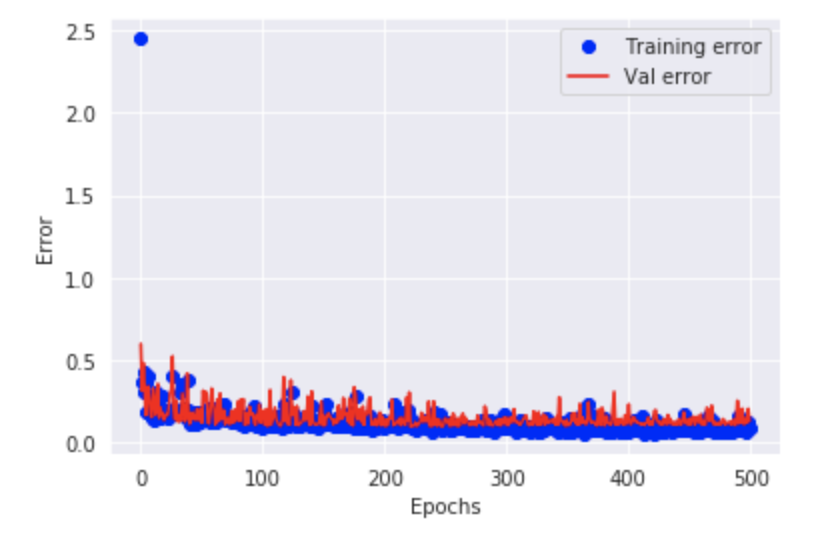
\includegraphics[width=0.48\textwidth]{acc.png}}
		\subfigure[The loss on the training set and validation set.]{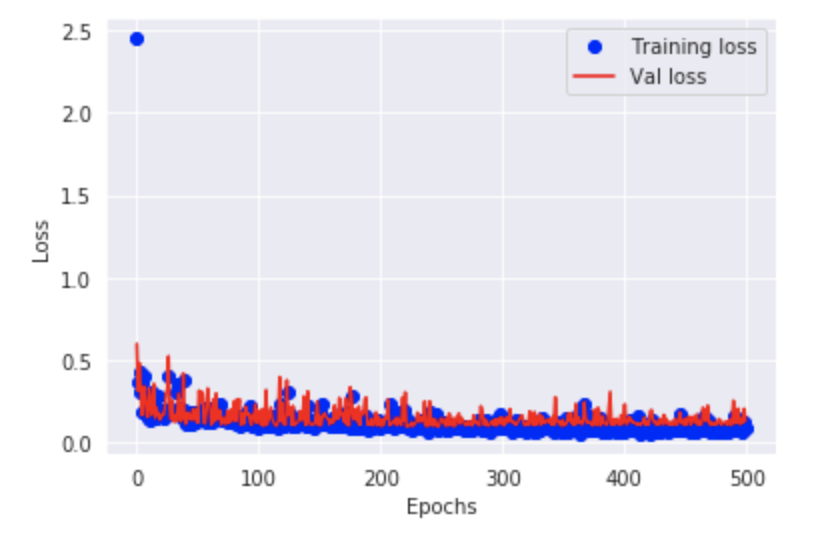
\includegraphics[width=0.48\textwidth]{loss.png}}
	\end{center}
	\caption{The convergence curves.}
	\label{fig:convergence}
\end{figure}
%---------------------------------Figure---------------------------------%





\section{Compared Methods}


\paragraph{Fully-connected neural network.}
We implemented a 3-layer fully-connected neural network.
The width of the layers (from bottom to top) are all 256, as output is linear.
The training and validation mean absolute error are respective 0.0907 and 0.09686


\paragraph{Random Forest Regressor.}
We use the random forest regressor model provided by SKlearn, as well as cross validation method. We set folds as 5, and report the mean score of mean absolute error. The mean score of this model is 0.1041. (Result is in Model 3)

\paragraph{Bayesian Regression.}
We use the linear model, BayesianRidge model provided by SKlearn. as well as cross validation method. We set folds as 5, and report the mean score of mean absolute error.
The mean score of this model is 0.08393. (Result is in Model 3)

\paragraph{Baseline Model}

We also fit our model with some baseline model. Following are the results.
\begin{itemize}
	\item 
	LASSO Regression.
	Alpha is 0.0005, Random state is 1, the score is 0.1115 (standard deviation is 0.0074)
	\item 
	Elastic Net Regression.
	Alpha is 0.0005, l1 ratio is 0.9, random state is 3, the score is 0.1116 (standard deviation is 0.0074)
	\item
	Kernel Ridge Regression
	Alpha is 0.6, kernel is 'polynomial', degree is 2, coefficient is 2.5. The score is 0.1153 (standard deviation is 0.0075)
	\item
	Gradient Boosting Regression
	n estimators is 3000, learning rate is 0.05, max depth is 4. The score is 0.1177 (standard deviation is 0.0080)
	\item
	XGBoost
	Gamma is 0.0468, learning rate is 0.05, max depth is 3,The score is 0.1161 (standard deviation is 0.0079)
	\item
	LightGBM
	Objective is 'regression',num leaves is 5, learning rate is 0.05, n estimators is 720, max bin is 55. The score is 0.1157 (standard deviation is 0.0067)
\end{itemize}



\section{Outcome}


We participated in an active competition.
Our score is 0.11555 in the public leaderboard (private leaderboard not available).
We rank 506/5384 in the public leaderboard.
(We just have one member in our team)
The screenshots are in Figure~\ref{fig:leaderboard}.





%---------------------------------Figure---------------------------------%
\begin{figure}
	\begin{center}
		\subfigure[Private leaderboard.]{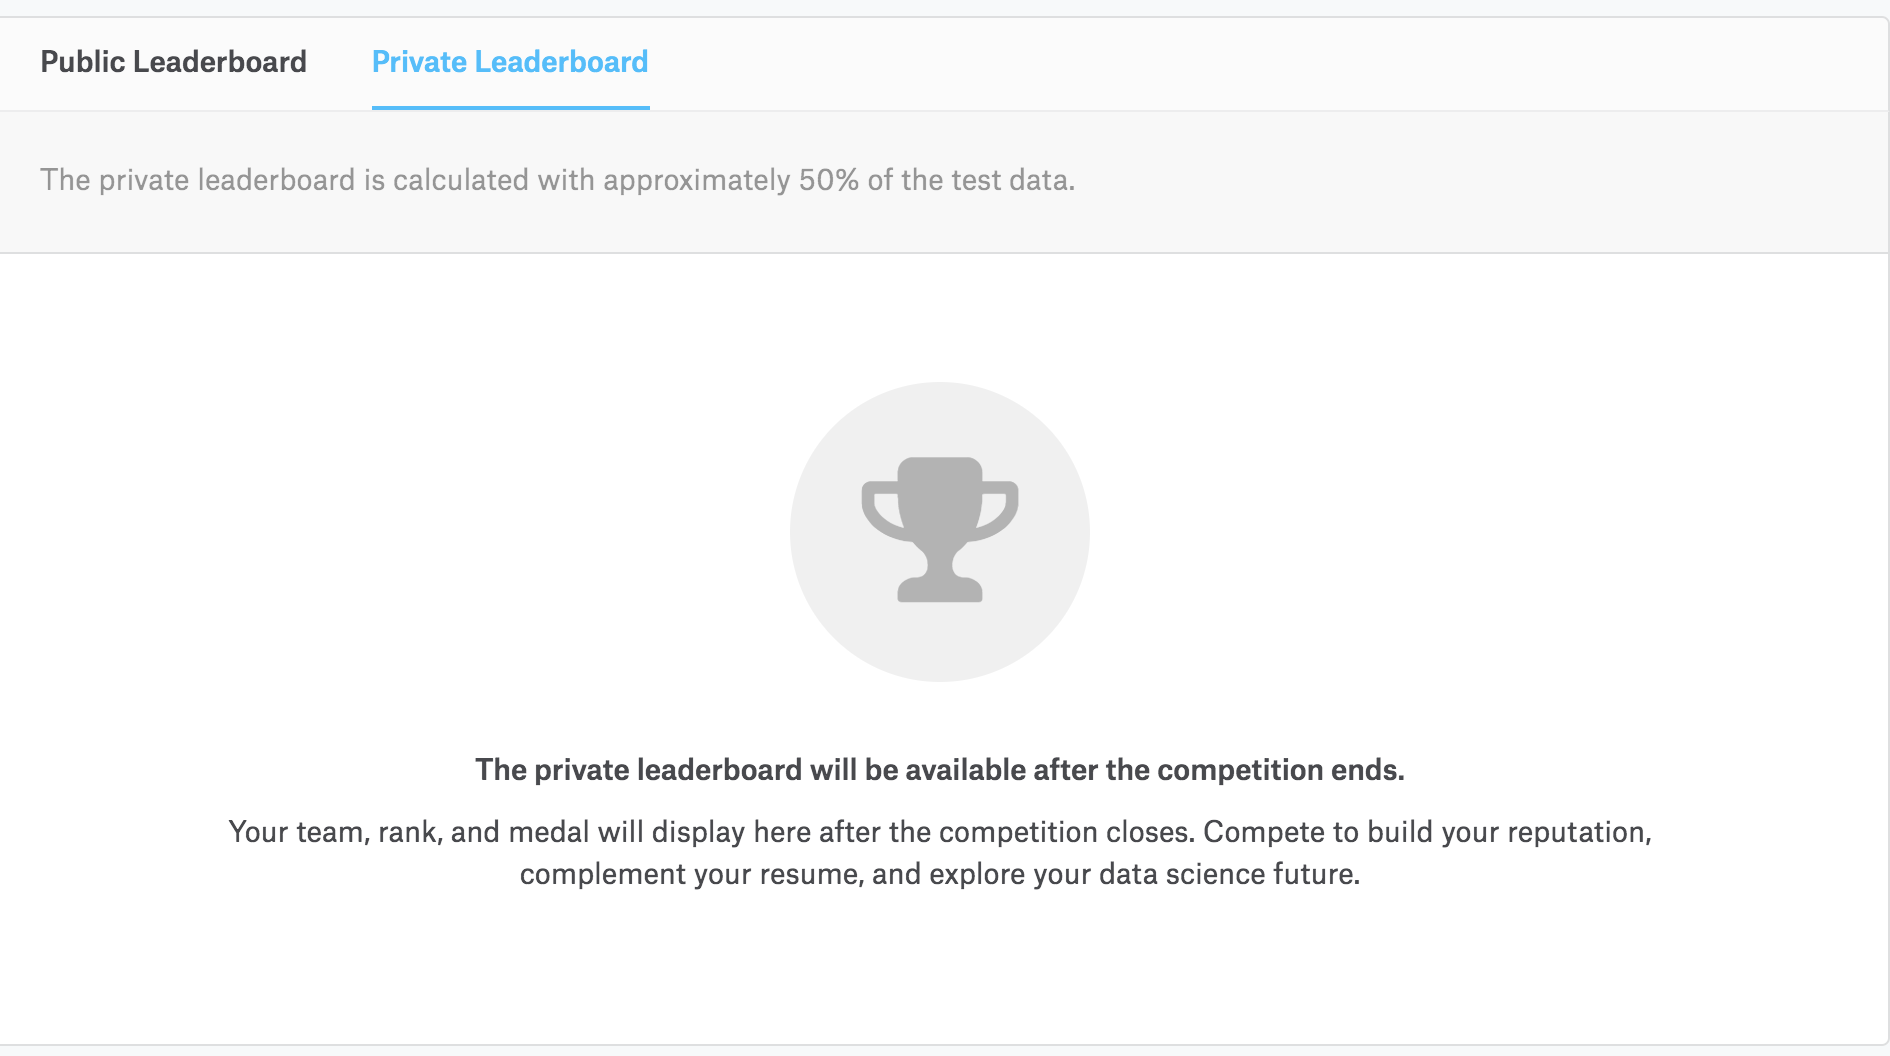
\includegraphics[width=0.48\textwidth]{private.png}}
		\subfigure[Public leaderboard.]{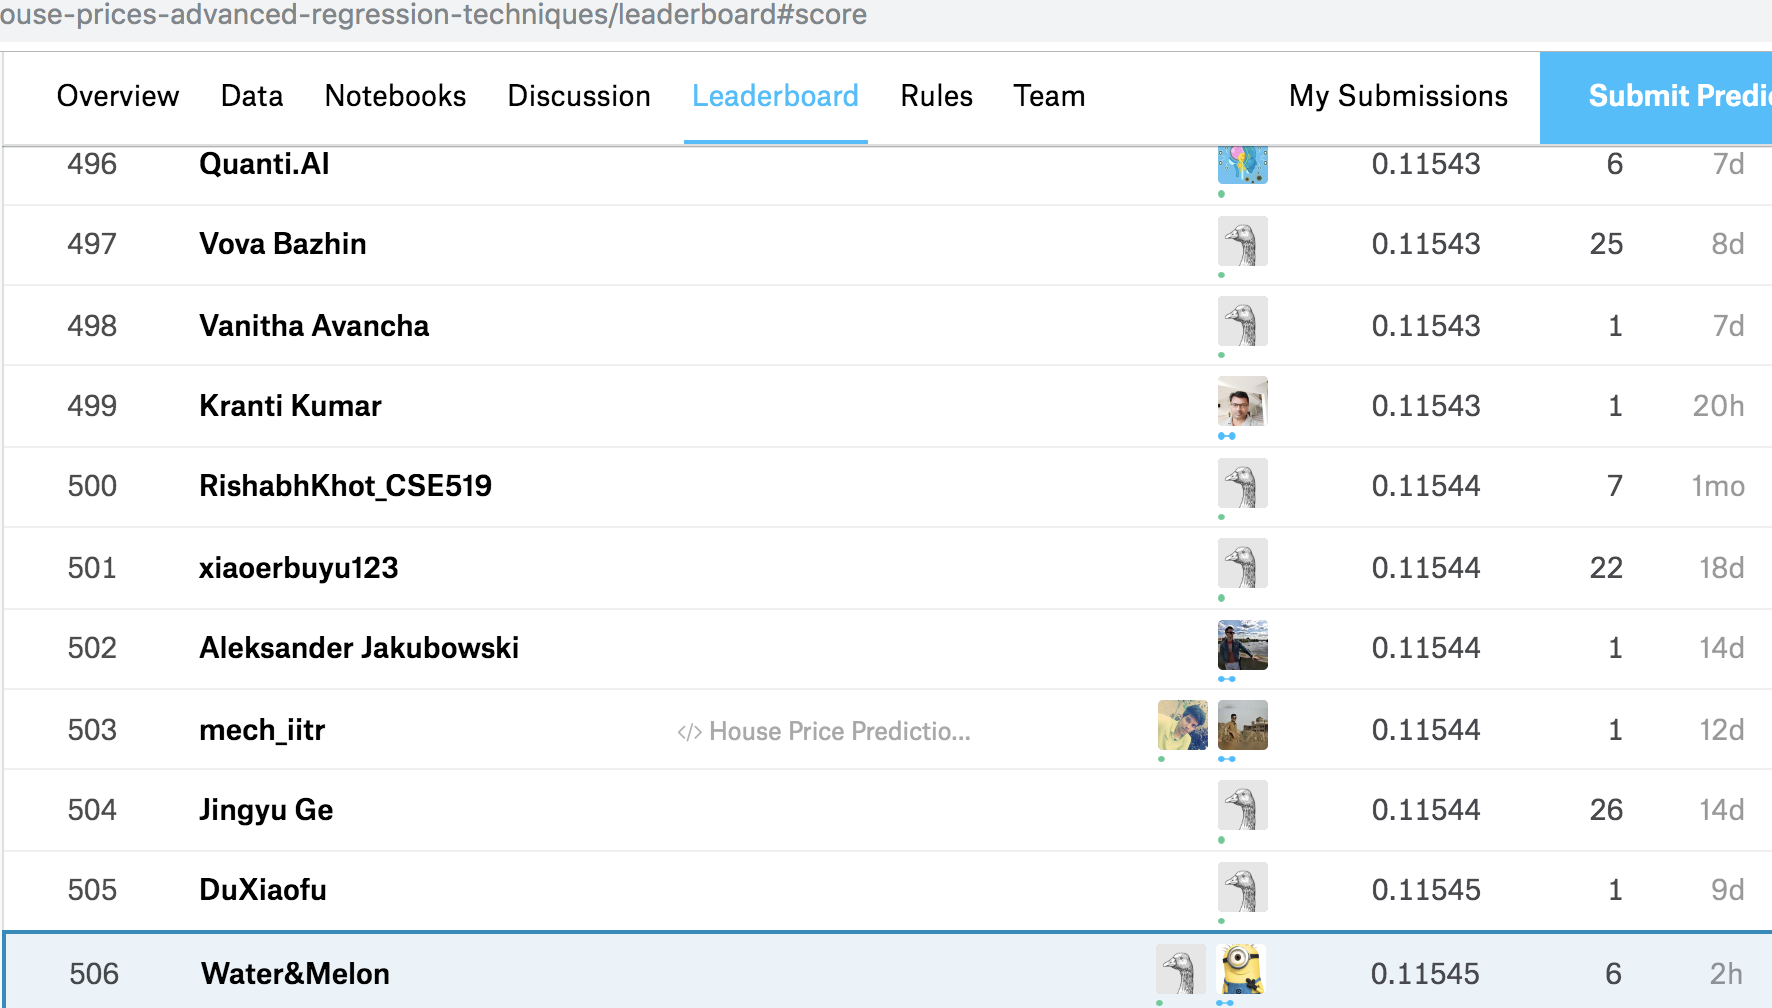
\includegraphics[width=0.48\textwidth]{public.png}}
	\end{center}
	\caption{Our rankings in the leaderboard.}
	\label{fig:leaderboard}
\end{figure}
%---------------------------------Figure---------------------------------%



%\vspace{3mm}
%\begin{lstlisting}
%import numpy
%
%def rfm(x, s, sigma):
%	n, d = x.shape
%	a = numpy.random.standard_normal((d, s)) / sigma
%	b = numpy.random.rand(1, s) * (2 * numpy.pi)
%	c = numpy.dot(x, a) + b
%	h = numpy.cos(c) * numpy.sqrt(2/s)
%	return h
%\end{lstlisting}
%\vspace{3mm}

%\newpage
\bibliographystyle{plain}
\bibliography{reference}


\end{document}